\hypertarget{obsah-kurzu}{%
\chapter{Obsah kurzu}\label{obsah-kurzu}}

V~poslední kapitole si představíme vytvořený online kurz pro výuku datové analytiky. Tuto část dělíme do tří vzájemně provázaných částí, z~nichž každá reflektuje odlišnou oblast návrhu a~implementace online kurzu.

\hypertarget{prux16fchod}{%
\section{Průchod}\label{prux16fchod}}

V~první částí se zaměříme na průchod kurzem, popíšeme si tedy, jak je kurz navržen po strukturální stránce a~jakým způsobem student prochází jednotlivými částmi.

\textbackslash begin\{figure\}{[}ht{]}\\
\centering 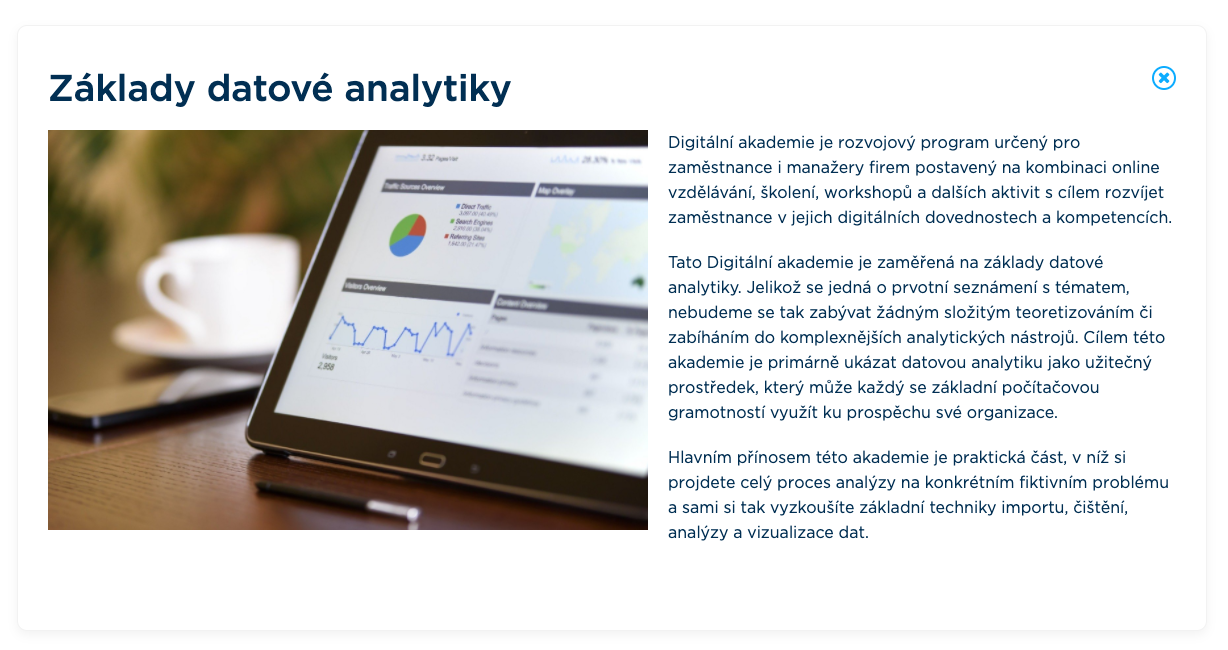
\includegraphics[width=.9\textwidth]{kurz-uvod}\\

\caption{Úvodní obrazovka s~představením kurzu (v~prostředí Digiskills digitální akademie)}

\} \label{kurz-uvod} \textbackslash end\{figure\}

\hypertarget{komponenty}{%
\section{Komponenty}\label{komponenty}}

\hypertarget{moduly}{%
\section{Moduly}\label{moduly}}
